\documentclass{article}

% Language setting
% Replace `english' with e.g. `spanish' to change the document language
\usepackage[english]{babel}
\usepackage{float}

% Set page size and margins
% Replace `letterpaper' with `a4paper' for UK/EU standard size
\usepackage[letterpaper,top=2cm,bottom=2cm,left=3cm,right=3cm,marginparwidth=1.75cm]{geometry}

% Useful packages
\usepackage{amsmath}
\usepackage{graphicx}
\graphicspath{{images_final/}}
\usepackage[colorlinks=true, allcolors=blue]{hyperref}

\title{Final Report}
\author{Group 2: Chenfeng Li, Nathan Suhr, Qian Liu}
\date{December 7, 2023}

\begin{document}
\maketitle


\section{Introduction}


% introduction section for Final Report:
Studying how diseases spread among populations is important for deciding public health policies and interventions. Our project constructs an agent-based model for a simulated disease to monitor how illnesses behave and spread within simulated populations. The model was built to simulate COVID-19's effect on a population; However, our model can work for any virus. One can use our model to simulate the propagation of disease assuming many parameters and levels of preparedness. For example, simulate a quickly mutating disease, an illness for which a vaccine already exists, and assess the effects of mask-wearing. Such a model would help researchers, and officials predict the damage of a disease and prepare appropriately beforehand.\\ \indent Our simulation presents data by tracking the number of people healthy, recovered, infected, and dead, as well as tracking the positions of each person over time. To aid in the versatility of our model, the user can set many parameters. These include the mutation rate of the virus, the percentage of people initially infected, the number of people overall, the space between them, as well as the percentage of people masked and vaccinated. Additionally, the user can predetermine how people move relative to one another. For example, the user can dictate that people will tend to gather or move away. With many ways to customize, one can set the disease simulation specific to their pandemic and can use the data to decide on a response. \\ \indent
The primary goal of our simulation is to model the trajectory of a disease's propagation for as many different parameters as possible. This is done by accounting for as many factors as possible and by using real-world data to aid in the accuracy of our model. Initially, we used real world data to simulate the effects of Covid-19 on a population. We used Study Shows Probability of Getting Covid for Mask Wearers vs. Non-Mask
Wearers." by Bhavana Kunkalikar to gather data about the likelihood of a mask blocking infection from Covid-19. Additionally, we used “Coronavirus: What Is Herd Immunity and Are You Protected If You Have
Antibodies?” by Stephanie Watson in order to decide how to implement the vaccine into our model. Finally, we used “Unveiling the Impact of Covid-19 Vaccines: A Meta-Analysis of Survival Rates among Patients in the United States Based on Vaccination Status.” by Ikeokwu et al. to decide on the rate which the vaccine would prevent death from Covid-19. However, we ultimately decided to let the user adjust all of this data to their liking so that our model could be more versatile and apply to more viruses than just Covid-19. 
%end of introduction



\section{Numerical Methods and Packages}

%Section for final report:
To use our model, one must provide the size of the grid in which the people are placed, the number of time steps to be simulated, the number of people, and the amount of people initially infected. Then, each person is initialized at a random position on the grid. After this, the distance for which the infection rate of the virus is .01\% is then calculated. To do this, we compute the optimization solution with the initial guess equal to 1. This is performed via scipy.optimize.fsolve for the distance function the user specified for their virus. At each time step, every living person moves. If the movement tendency is set to random, the person's movement will be randomly picked from one of four options. They can either go up, down, left or right. However, they cannot go in a particular direction if doing so would move them out of bounds or overlap. Our model also includes other movement strategies which are gather, stay away, and party.\\ 
\indent As for the status of people, if two people are within distance for the infection to be possible, this will move these individuals to the susceptible category if they are healthy. Once susceptible, they will have a random chance to be infected and a random chance for their mask to save them from infection. The chance for the mask to save them is the chance of the mask\_penetration parameter of the virus that the user specifies The probability of infection depends on the distance and is determined using the distance function the user specified. Once infected the user has a chance of dying, depending on the mortality rate that the user set for their virus. If the user is meant to die during this time step but have taken the vaccine, they will be given a chance to live. This chance depends on the vaccine\_effectiveness parameter which the user sets for their virus. All of these chances are calculated by drawing a random number between 0 and 1 and deciding an outcome based on whether this number is greater or less than the chances which are provided by the user. The random numbers are generated using numpy.random.random. To record the status for each person on a given time step, a deep copy of a list is used via the deep copy from the copy package. The deep copy avoids pointers and references so that no status will be altered upon appending another. 

\indent The original way to detect the status of people is by running a nested loop to find all (healthy, infected) pairs. To speed up the process of our simulation, the KD-tree can be implemented in the detect step. Applying the KD-tree helps partition the whole space into k-dimensional space. In our setting, the KD-tree will separate the whole population into K-groups based on the distance between each individual, so the closest people will be divided into a group and there will be k=10 groups in the whole simulated population by default. 
%end of section

\section{Structuring of src}

%Section for Final Report:
Our src folder will contain a file which is Disease\_Model\_Source\_Code\_Final.py. This file will contain all of our source code and will allow the user to use our model if they import it. The "Disease Model Examples Final Part 1" and "Disease Model Examples Final Part 2" in the examples folder can be run to see some examples of our simulation. In order to run the model, the user must utilize the Simulation class. This class takes in board size, number of time steps, number of people, percentage of people initially infected, and virus type as required parameters. The virus is a dictionary, with the parameters being "healthy", "infected", "mutation\_rate", "mask\_penetration" and "vaccine\_effectiveness". The "healthy" parameter is a function which is the probability of a healthy person being infected by a carrier. The "infected" parameter is the fatality rate. The last three parameters are meant to be from 0 to 1 and determine how fast the virus mutates, the effectiveness in mask wearing to deter infection and how well the vaccine can prevent mortality. The mutation rate affects our simulation by introducing a chance that recovered people can be reinfected. The higher the mutation rate is, the higher this chance is.\\ \indent Optional parameters of the Simulation class include "strategy", the seed, the percentage of people who have a mask, the percentage of people vaccinated, and finally the mutation rate of the virus. To perform the actual simulation, one must use the simulate helper function for the Simulation Class. One can see the current board by using the board helper function. To visualize the output, the user can use the plot or animate helper functions. The "strategy" parameter has four options which are "gather", "stay away", "random" and "party" and depending on which of the four is chosen, the people in the simulation will move according to that choice. For example, if "stay away" is chosen, 90\% of movements will maximize the distance between one another and 10\% of the movements will be random. \\ \indent This file also contains another important class which is called "Person". The "Person" class stores a list of attributes about each individual in the simulation. It stores the health status, the position of the person, and whether or not they have a mask or vaccine. Additionally, there is a helper function that computes the distance between this person and another point on the grid. The Simulation class first initializes the board and then initializes the people. Then, a random initial position is assigned for each person. The "move" helper function moves each person according to the strategy parameter and the "detect" decides which healthy people will be infected during this time step. It also decides whether those who are already infected will recover, die, or remain infected. The "record\_step" function records the status of each person during the time step so that this data can be plotted later. Lastly, the "one\_step" function simulates one-time step of our simulation. It also converts people from recovered to healthy, meaning that they are susceptible to reinfection, according to the mutation rate parameter. 


\section{Tests}

We have multiple tests for both the person class and the simulation class. For the person class, we have four tests. The first test checks if the person is initialized with the correct properties. We set "position=[1,1], status='healthy', mask=1" and check if the properties of the person after the initialization are the same as what we set. The second checks after a person becomes infected, whether the status of this person is updated as infected correctly. The third test is similar to the second one; it focuses on the update of the position. The last test for the person class is to test if the distance between two given persons is calculated correctly. For example, the Euclidean distance between a person at [1,1] and another person at [0,0] should be the square root of two; this is what we check in the test. \\
\indent We have another three tests for the simulation. Our first test helps check if the simulation is initialized with the correct properties. In more detail, we check if the value of board\_shape, ts, num\_people is the same as what we set and if the current\_ts is 0, the start of the time step. We also check if the status is initialized correctly based on calculating the expected number of infected people and dead people. Besides, since we set the moving strategy to be random, we also test if two simulations with different seeds generate people with different positions at the beginning. The next test ensures nobody moves out of the bounds of the board and that no two people are overlapping. The last test checks if the status of each time step is recorded and the list is updated with the correct length.\\ 

\section{Results}

In order to see how the movement strategies of the people in the simulation affected the transmission of the virus, we set a trial using each of these strategies. To best gauge the effect of each movement strategy, mutation rate, mask, and vaccination rates aren't considered.
\begin{figure}[H]
    \centering
    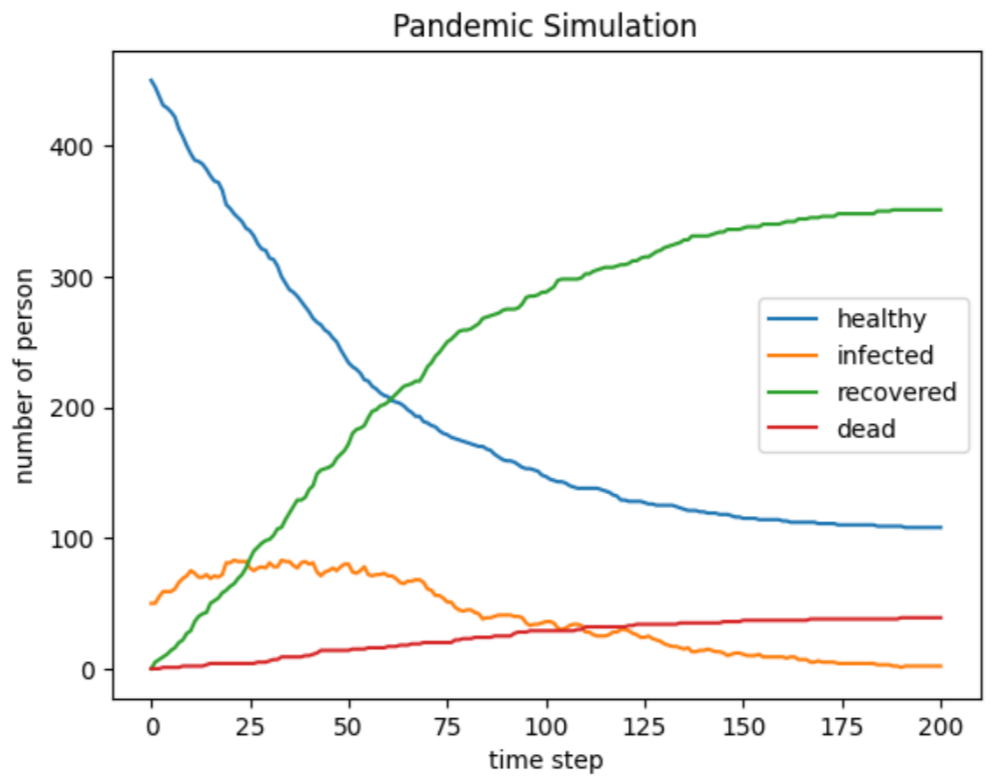
\includegraphics[width=.6\linewidth]{figure1.png}
    \caption{500 * 500 board with 1000 people, (10\% infected), 100 time steps, random movement}
    \label{fig:enter-label}
\end{figure} 
\begin{figure}[H]
    \centering
    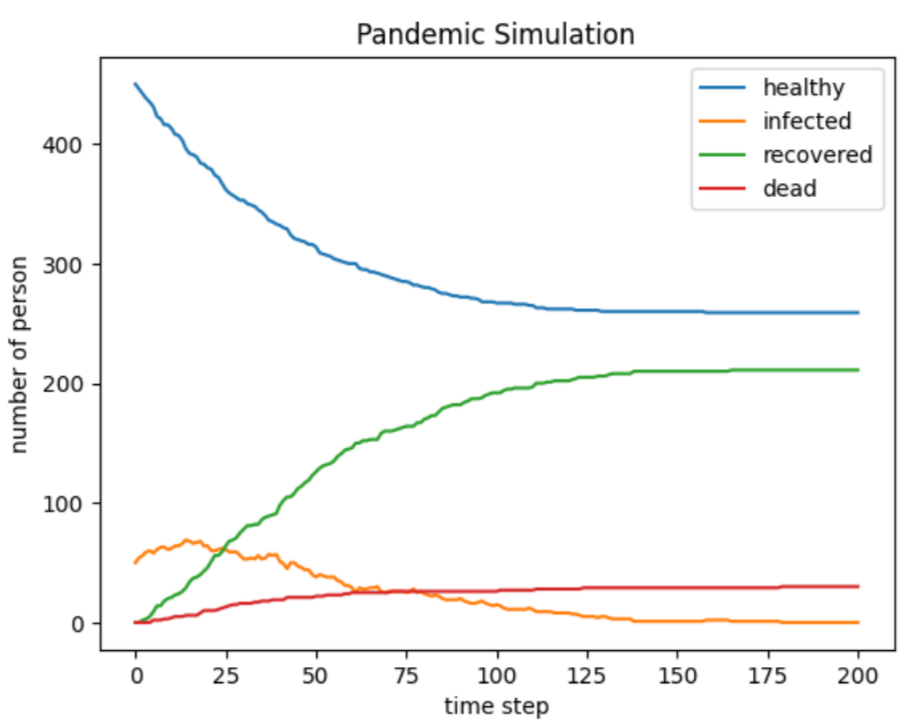
\includegraphics[width=.6\linewidth]{figure2.png}
    \caption{500 * 500 board with 1000 people, (10\% infected), 100 time steps, "stay away" movement}
    \label{fig:enter-label}
\end{figure} 
As we can see, when people tend to stay away from each other, the virus transmission is much lower. This is evident in each of the plot by noticing that the curve of healthy people falls much faster in figure 2. Additionally, at the end of the figure 1 time steps, many less people in total are infected. Another way to visualize the simulation in figure 2 is via the 
\href{https://github.com/UChi-ComPy23/group-project-group2/blob/main/doc/final/stayaway.gif}{stay away} gif. One can see the people, represented by points, doing their best to spread apart from one another
\begin{figure}[H]
    \centering
    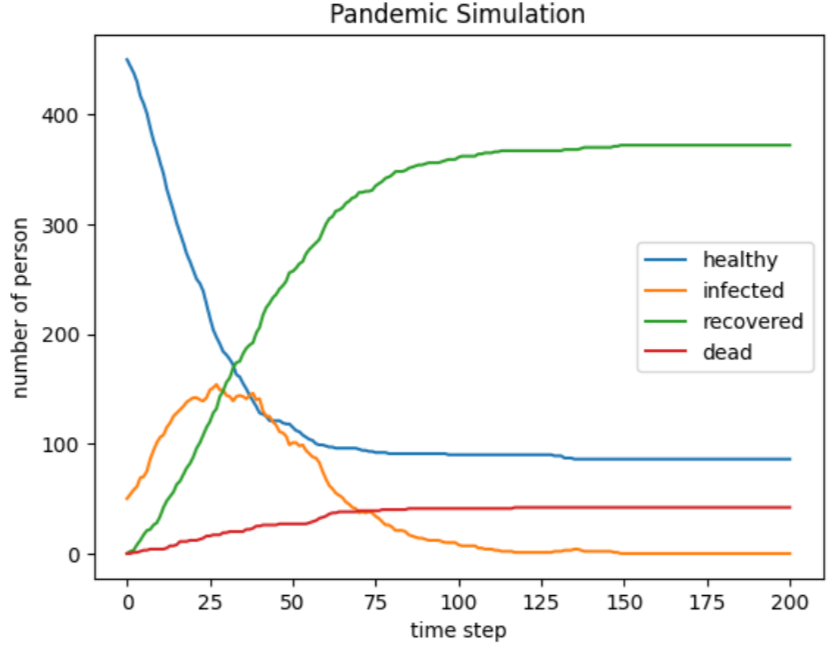
\includegraphics[width=.6\linewidth]{figure3.png}
    \caption{500 * 500 board with 1000 people, (10\% infected), 100 time steps, "gather" movement}
    \label{fig:enter-label}
\end{figure}
In the first two figures, the infection curve is mostly similar. However, comparing these two to figure 3, one can see the infection rate spikes much higher when people tend to gather. Additionally, from figure 3, we can see that the number of healthy people drops much faster than the other two simulations. The tendency to gather can be visualized with the
\href{https://github.com/UChi-ComPy23/group-project-group2/blob/main/doc/final/gather.gif}{gather} gif.
\begin{figure}[H]
    \centering
    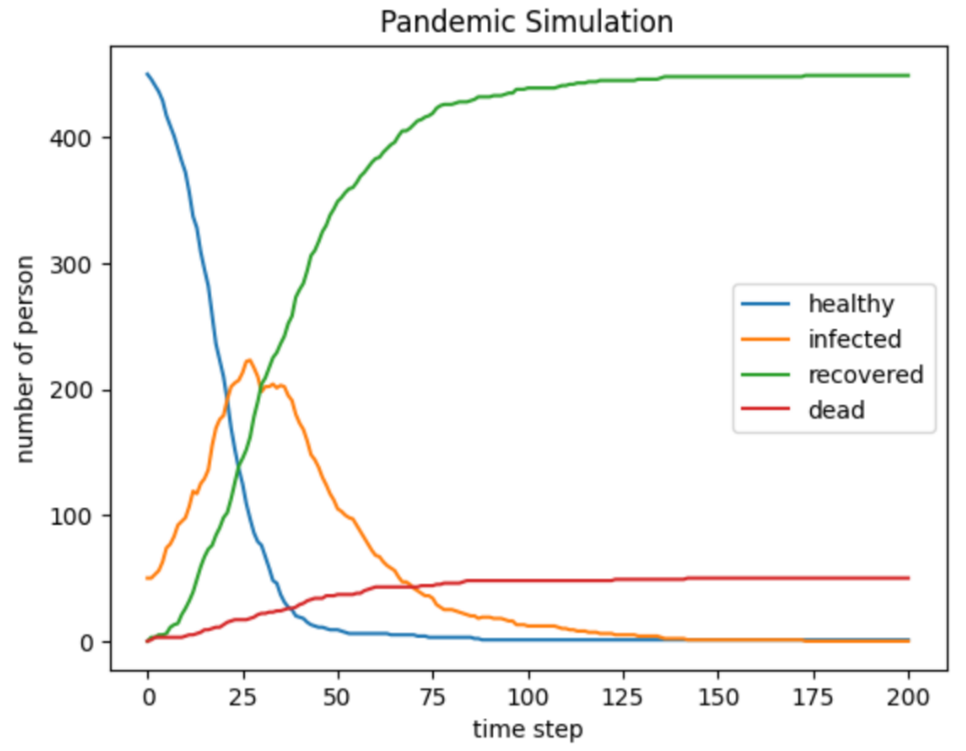
\includegraphics[width=.6\linewidth]{figure4.png}
    \caption{500 * 500 board with 1000 people, (10\% infected), 100 time steps, "party" movement}
    \label{fig:enter-label}
\end{figure}
Finally, from figure 4, one can see that the number of healthy people drops the fastest and the infection curve reaches a higher rate than any of the other figures. This is because the "party" movement option has people congregate more than any other movement option. Though the version of the virus used for these simulations is relatively nonlethal, one can derive from the figures that increased congregation leads to much higher infection rates initially. The \href{https://github.com/UChi-ComPy23/group-project-group2/blob/main/doc/final/party.gif}{party} gif most clearly shows the people's tendency to congregate. One can see that this leads to significantly higher infection rates.\\\\
For this next simulation, all conditions are kept the same, except the virus mutation rate is set to .2 instead of 0 and the random movement is used. 
\begin{figure}[H]
    \centering
    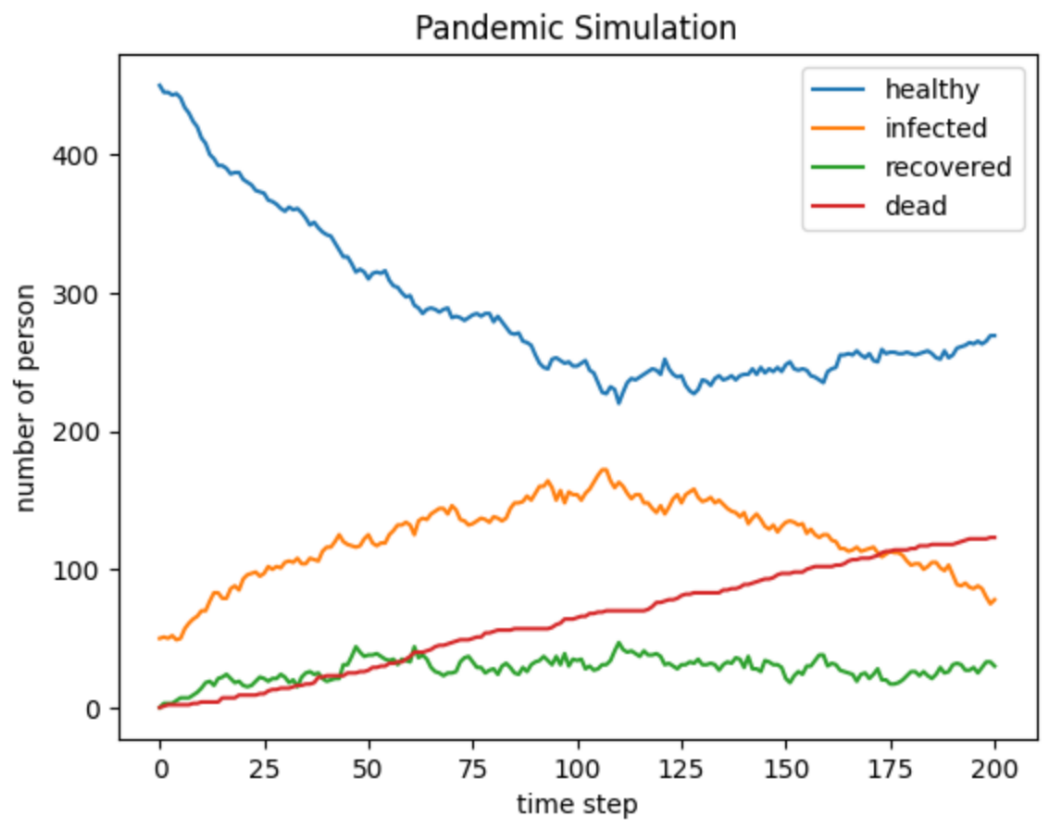
\includegraphics[width=.6\linewidth]{figure5.png}
    \caption{500 * 500 board with 1000 people, (10\% infected), 100 time steps, .2 mutation rate}
    \label{fig:enter-label}
\end{figure}
By viewing figure 5, one can see that the mutation rate has greatly reduced the amount of people who are recovered, and are not susceptible to infection. This is especially noteworthy because, if every member of a population is "recovered", this indicates herd immunity. However, from this simulation, we can see that herd immunity will not be reached if the virus mutates at this rate. Another noteworthy result from this simulation is that the total number of deaths at the end of the time steps is significantly higher than any of our other simulations. As opposed to the movement strategies which mostly affected the rate of infection, the mutation rate seems to affect primarily the recovery rate and death toll. \\\\

Next, to simulate the effect of mask wearing, we keep the conditions from figure 5 but add a 20\% mask wearing rate as well as a mask penetration rate of 0.2 so that the masks are reasonably effective. 
\begin{figure}[H]
    \centering
    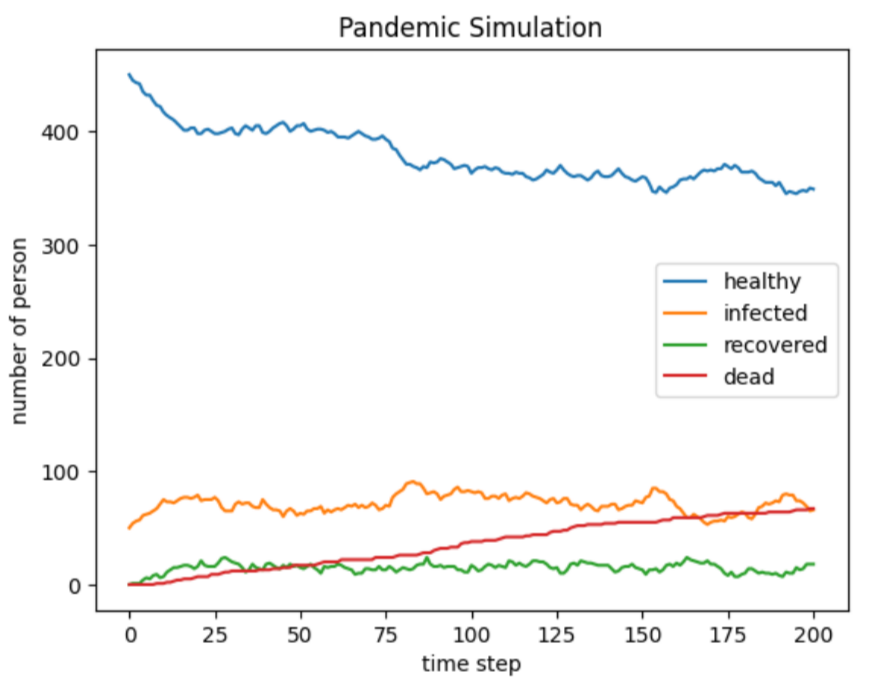
\includegraphics[width=.6\linewidth]{figure6.png}
    \caption{500 * 500 board with 1000 people, (10\% infected), 100 time steps, .2 mutation rate, .2 mask and mask penetration rate}
    \label{fig:enter-label}
\end{figure}
From figure 6, we can clearly see that mask wearing was an extremely effective deterrent of disease transmission, even when only 20\% of the population wore a mask. The most notable way this can be seen is by observing the curve of healthy and infected individuals. Unlike that of figure 5, the health curve for figure 6 barely dips. Note that that isn't necessarily representative of the number of people who have never gotten the disease since the mutation rate is nonzero. However, comparing this with figure 5, one can see that transmission was extremely diminished. Additionally, even in a situation where previously infected people can get the disease again, the masks will be more effective for these people. This is because it will lower the chances of contracting the disease both initially and at any other instance. Thus, in a situation in which herd immunity cannot be naturally achieved, masks may be among the best strategies for social safety since the death toll was significantly lower in figure 6. \\\\
Finally, we test the vaccine. For our vaccine, we assumed a very effective vaccine with mass adoption of this vaccine. We also assumed nobody had a mask so that we could see purely the effects of the vaccine. 
\begin{figure}[H]
    \centering
    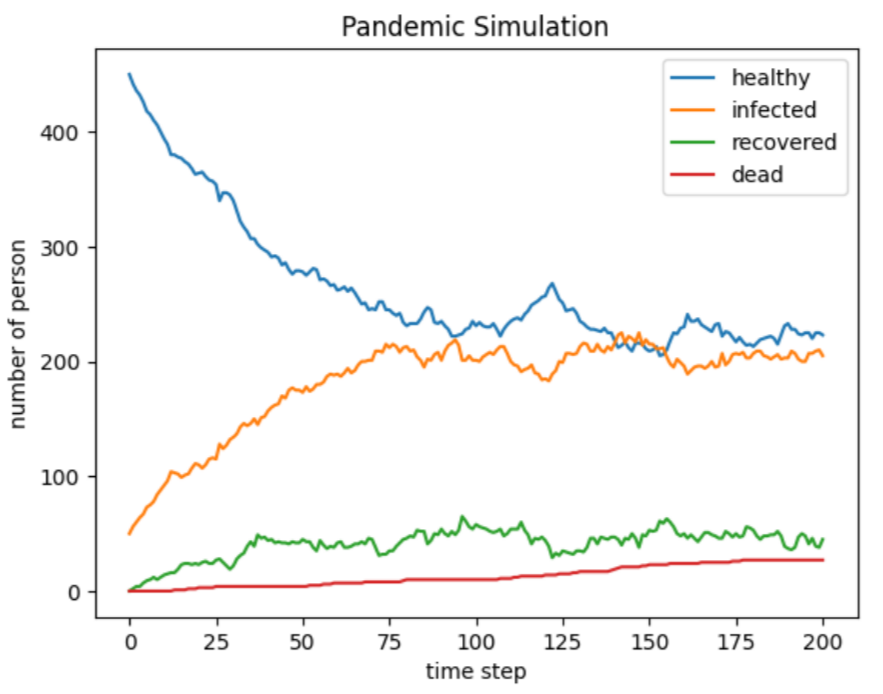
\includegraphics[width=.6\linewidth]{figure7.png}
    \caption{500 * 500 board with 1000 people, (10\% infected), 100 time steps, .2 mutation rate, .8 vaccine rate and vaccine effectiveness}
    \label{fig:enter-label}
\end{figure}
The way our vaccine is implemented is meant to lessen the severity of the symptoms of the disease. In our actual model, this is represented as a much greater chance for infected individuals to survive. From viewing figure 7, we can see that the vaccine was especially effective in lowering the mortality rate. Even in an environment with no masks and thus much more infection, the mortality rate was lower in figure 7 than that of figure 6. Therefore one can infer from the data that masks in conjunction with the vaccine is the most effective way to maintain safety of the populous. 
\\\\ \\\\ \\\\ \\\\ \\\\ \\\\ \\\\ \\\\ \\\\ \\\\ \\\\ \\\\ \\\\ \\\\
\section{References}
Kunkalikar, Bhavana. “Study Shows Probability of Getting Covid for Mask Wearers vs. Non-Mask Wearers.” Https://Www.News-Medical.Net/, 4 Aug. 2022, www.news-medical.net/news/20220802/Study-shows-probability-of-getting-COVID-for-mask-wearers-vs-non-mask-wearers.aspx. \\\\
Watson, Stephanie. “Coronavirus: What Is Herd Immunity and Are You Protected If You Have Antibodies?” WebMD, WebMD, 2023, www.webmd.com/covid/coronavirus-immunity-reinfection. \\\\
Ikeokwu, Anderson E, et al. “Unveiling the Impact of Covid-19 Vaccines: A Meta-Analysis of Survival Rates among Patients in the United States Based on Vaccination Status.” Cureus, U.S. National Library of Medicine, 10 Aug. 2023, www.ncbi.nlm.nih.gov/pmc/articles/PMC10492612/. 


\end{document}